\documentclass[10pt,a4paper, twocolumn]{article}
\usepackage[utf8]{inputenc}

\usepackage{tikz}

\usetikzlibrary{calc}
\begin{document}

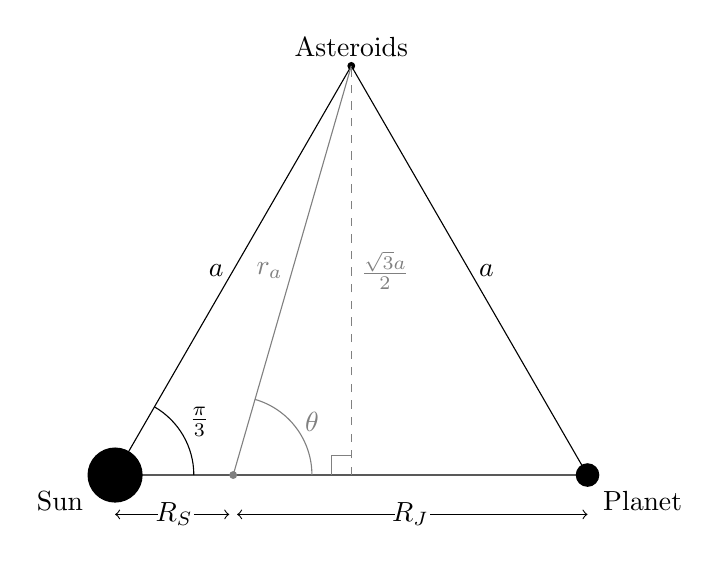
\begin{tikzpicture}
\draw (0,0) -- (6,0) -- (3, {6*sin(60)} ) node[above]{Asteroids} node[midway,right]{$a$} -- cycle node[midway,left]{$a$};
\draw  (1,0) arc (0:60:1cm)  ;
%\node [label={[shift = {(10mm,5mm)}]{$\frac{\pi}{3}$}}] {};
\node [label={[shift = {(13:11mm)}]{$\frac{\pi}{3}$}}] {};
\node [label={[shift = {(-7mm,-7mm)}]{Sun}}] {};
\node [label={[shift = {(67mm,-7mm)}]{Planet}}] {};


\fill[black] (0,0) circle (3.5mm);% node[anchor=north west] {Sun};
\fill[black] (6,0) circle (1.5mm);
\fill[black] (3, {6*sin(60)} ) circle (0.5mm);

\fill[gray] ({6*(1/4)}, 0) circle (0.5mm);
\draw[gray] ({6*(1/4)}, 0) -- (3, {6*sin(60)} ) node[midway,left]{$r_{a}$};
\draw[dashed, gray] (3, 0) -- (3, {6*sin(60)} )node[midway,right]{$\frac{\sqrt{3}a}{2}$};
\draw[gray]  ({6*(1/4) + 1}, 0) arc (0:{atan(4*sin(60))}:1cm)  ;
\node [label={[gray, shift = {(25mm,3mm)}]$\theta$}] {};
\draw[gray] (2.75,0) -- (2.75, 0.25) -- (3, 0.25);

\draw[arrows=<-](0,-0.5)--(0.55,-0.5);
\node at (0.75, -0.5) {$R_S$};
\draw[arrows=->](1,-0.5)--(1.45,-0.5);

\draw[arrows=<-](1.55,-0.5)--(3.55,-0.5);
\node at (3.75, -0.5) {$R_J$};
\draw[arrows=->](4,-0.5)--(6,-0.5);

%\draw[arrows=<-](0,-1)--(2.88,-1);
%\node at (3, -1) {$a$};
%\draw[arrows=->](3.1,-1)--(6, -1);

\end{tikzpicture}


%planet mass is one third of solar mass 
	
\end{document}